\documentclass[11pt]{article}
\usepackage[margin=1in]{geometry}
\usepackage{booktabs}
\usepackage{amsmath}
\usepackage{siunitx}
\usepackage{pgfplots}
\pgfplotsset{compat=1.17}
\usepackage{hyperref}
\usepackage{xcolor}
\hypersetup{colorlinks=true,linkcolor=blue,urlcolor=blue}

\title{Pioneer.jl SearchDIA Allocation Analysis}
\author{Allocation-reduction effort --- branch \texttt{perf/alloc-diagnostics}\\(off \texttt{perf/combined-allocations})}
\date{2026-06-24}

\begin{document}
\maketitle

\begin{abstract}
This document tracks the memory-allocation analysis of Pioneer's \texttt{SearchDIA}
pipeline. Benchmark: \texttt{MtacYeastStandard3M} (3 Thermo Astral DIA files, 3-min
gradient) searched against the \texttt{yeast\_May7-2026\_bitvec\_10.poin} library
($\sim$619k target precursors), at 36 threads unless noted. All numbers are warm
(post-JIT) unless stated. ``Allocation'' means cumulative heap bytes
(\texttt{gc\_bytes} / \texttt{@timed.bytes}, summed across threads), which is GC
churn, \emph{not} peak working set (RSS).
\end{abstract}

\section{Methodology}
Three complementary instruments were used:
\begin{itemize}
  \item \textbf{\texttt{@timed} per-phase} (exact): true total bytes per pipeline phase.
  \item \textbf{\texttt{@alloc\_bucket}} (exact, env-gated \texttt{PIONEER\_DIAG\_ALLOC}):
        \texttt{gc\_bytes} delta around named Main Search sub-steps.
  \item \textbf{\texttt{Profile.Allocs}} (sampled, rate $10^{-4}$): attributes each
        sampled allocation \emph{event} to its leaf source line and to the phase
        (\texttt{SearchMethods/}$\langle X\rangle$) its stack passes through.
\end{itemize}
\textbf{Important caveat.} \texttt{Profile.Allocs} samples allocation \emph{events},
so it pinpoints frequent \emph{small} allocations but \emph{under-counts rare large}
ones (a single multi-GB \texttt{resize!} is one event, usually missed). Hence the
sampled per-line totals are much smaller than the exact \texttt{@timed} phase totals;
the two are used together (exact = ``how much per part'', sampled = ``which line churns'').

\section{Per-phase totals (exact, warm)}
Total warm allocation on the combined branch: \textbf{35.0\,GB} over 3 files.
\begin{center}
\begin{tabular}{lr}
\toprule
Phase & Mem Alloc (GB) \\
\midrule
\textbf{Main Search}            & \textbf{16.76} \\
Precursor Scoring               & 4.06 \\
Quantification \& Output        & 3.52 \\
Chromatogram Integration        & 2.54 \\
BitVec Calibration              & 2.14 \\
Protein Scoring                 & 1.98 \\
Parameter Tuning                & 1.86 \\
Spectral Library Loading        & 0.82 \\
Quadrupole Tuning               & 0.39 \\
Search Context Initialization   & 0.37 \\
Huber Calibration               & 0.34 \\
Protein Inference               & 0.25 \\
\bottomrule
\end{tabular}
\end{center}

\section{Main Search breakdown (exact \texttt{@alloc\_bucket}, per file)}
The post-deconvolution PSM table footprint is only \SI{0.264}{GB} (200 B/row),
rising to \SI{0.363}{GB} (275 B/row) after features --- so most per-file Main Search
allocation is churn, not data footprint.
\begin{center}
\begin{tabular}{lrrr}
\toprule
Sub-step & file 1 & file 2 & file 3 \\
\midrule
\textbf{library\_search (deconv)} & \textbf{6.61} & 0.55 & 0.52 \\
train\_lgbm\_and\_select\_best     & 0.88 & 0.93 & 0.88 \\
chromatogram\_features            & 0.50 & 0.53 & 0.50 \\
permute\_by\_precursor            & 0.30 & 0.31 & 0.30 \\
ms1\_lookup\_features             & 0.23 & 0.24 & 0.23 \\
prepare\_psm\_features            & 0.16 & 0.17 & 0.16 \\
scan\_competition\_features       & 0.02 & 0.03 & 0.02 \\
\bottomrule
\end{tabular}
\end{center}
\noindent\textbf{Key observation:} \texttt{library\_search} allocates \SI{6.6}{GB} on
file 1 but only $\sim$\SI{0.52}{GB} on files 2--3. The excess is \emph{one-time
per-thread buffer growth} that is reused across files (Section~\ref{sec:threadscale}).
The \emph{recurring} per-file Main Search cost is $\sim$\SI{2.7}{GB}, led by
\texttt{train\_lgbm} ($\sim$0.9), \texttt{library\_search} ($\sim$0.52),
\texttt{chromatogram\_features} ($\sim$0.5).

\section{Thread-scaling of the one-time deconv growth}\label{sec:threadscale}
To test whether the file-1 growth is per-thread buffer allocation, the search was run
on a \emph{single} file at varying thread counts. ``Ctx Init'' is the
\texttt{Search Context Initialization} phase (pure per-thread struct allocation);
``library\_search'' is the file-1 deconv bucket. ``r1'' = cold (first \texttt{SearchDIA}
in the process), ``r2'' = warm (second call; JIT already paid, fresh context so buffers
regrow).
\begin{center}
\begin{tabular}{rrrrrr}
\toprule
threads & CtxInit r1 & CtxInit r2 & libsearch r1 & libsearch r2 & r1$-$r2 (JIT) \\
\midrule
1  & 0.05 & 0.01 & 1.648 & 1.075 & 0.573 \\
2  & 0.06 & 0.02 & 1.748 & 1.176 & 0.572 \\
4  & 0.08 & 0.04 & 1.763 & 1.191 & 0.572 \\
8  & 0.12 & 0.08 & 2.440 & 1.868 & 0.572 \\
16 & 0.20 & 0.17 & 3.797 & 3.225 & 0.572 \\
32 & 0.37 & 0.33 & 6.505 & 5.933 & 0.572 \\
\bottomrule
\end{tabular}
\end{center}
All figures GB. \texttt{r1$-$r2} is constant ($\approx$\SI{0.57}{GB}) across all thread
counts: that is the thread-independent JIT compilation cost.

\begin{center}
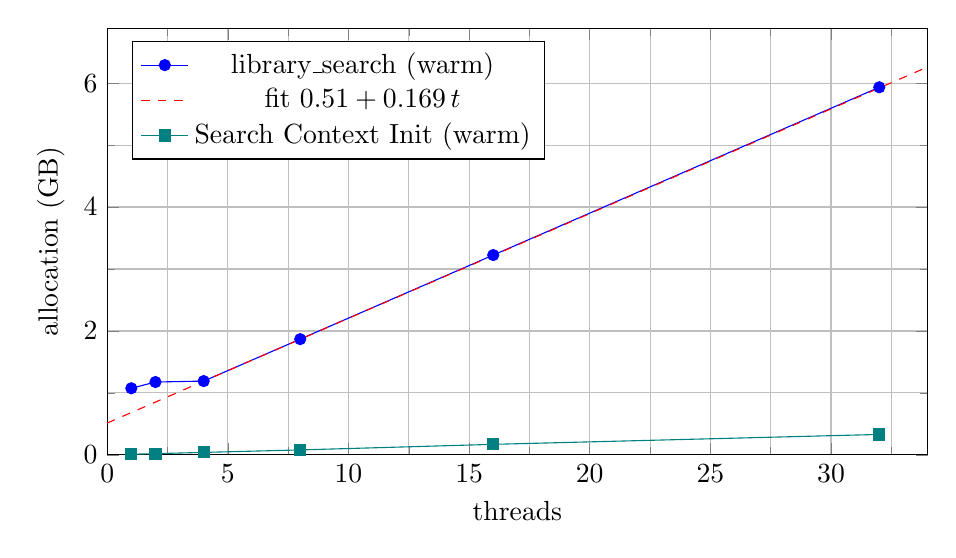
\begin{tikzpicture}
\begin{axis}[
    width=12cm, height=7cm,
    xlabel={threads}, ylabel={allocation (GB)},
    xmin=0, xmax=34, ymin=0,
    legend pos=north west, grid=both, minor tick num=1,
]
\addplot[mark=*,blue] coordinates {(1,1.075)(2,1.176)(4,1.191)(8,1.868)(16,3.225)(32,5.933)};
\addlegendentry{library\_search (warm)}
\addplot[dashed,red,domain=0:34] {0.514 + 0.169*x};
\addlegendentry{fit $0.51 + 0.169\,t$}
\addplot[mark=square*,teal] coordinates {(1,0.01)(2,0.02)(4,0.04)(8,0.08)(16,0.17)(32,0.33)};
\addlegendentry{Search Context Init (warm)}
\end{axis}
\end{tikzpicture}
\end{center}

\subsection{Decomposition and theory check}
\textbf{Search Context Init} (per-thread struct allocation) is linear through the
origin at \SI{10.3}{MB/thread} (slope of the warm series). The theoretical per-thread
footprint --- \texttt{Base.summarysize} of one \texttt{SimpleLibrarySearch} minus the
shared isotope splines --- is \textbf{\SI{11.05}{MB/thread}}. These match (the small
gap is shared/padding that \texttt{summarysize} attributes but marginal \texttt{gc\_bytes}
does not). The init buffers are dominated by \texttt{mass\_err\_samples}
($250{,}000$ samples) and the \texttt{precursor\_weights} \texttt{SparsePrecMap}
(sizehint $262{,}144$).

\textbf{\texttt{library\_search} (deconv)} fits (threads $\ge 4$):
\begin{equation}
\text{alloc}(t) \;\approx\; \underbrace{0.51\ \text{GB}}_{\text{thread-independent}}
\;+\; \underbrace{0.169\ \text{GB}}_{\text{per thread}} \cdot t .
\end{equation}
Interpretation:
\begin{itemize}
  \item The \textbf{constant \SI{0.51}{GB}} is the per-file, per-scan deconv work
        (DataFrame build, per-scan temporaries). It is data-bound, thread-independent,
        and \emph{recurs every file} --- exactly matching the $\sim$\SI{0.52}{GB}
        observed on files 2--3.
  \item The \textbf{\SI{0.169}{GB/thread}} is per-thread scratch \emph{growth} during
        deconvolution: the fused design matrix (\texttt{SparseArrayFused}/\texttt{Hs}),
        the scored/unscored PSM buffers and \texttt{FusedScratch} \texttt{resize!}-grow
        from their seed sizes (5000 / 256 elements) to the largest scan's complexity.
        It is paid \emph{once per \texttt{SearchDIA} call} (on file 1) and reused by
        later files.
\end{itemize}
At 36 threads this predicts $0.51 + 0.169\cdot 36 = \SI{6.6}{GB}$, matching the observed
file-1 \texttt{library\_search}.

\textbf{Per-thread totals:} $\sim$\SI{11}{MB} at init (matches theory) growing to
$\sim$\SI{180}{MB} of cumulative deconv allocation per thread. The growth is the
working set ($\sim$\SI{85}{MB}/thread after geometric \texttt{resize!}, $\sim 2\times$
in cumulative bytes) sized to the busiest scan.

\subsection{Consequences}
\begin{itemize}
  \item The one-time growth is \textbf{strongly thread-dependent} ($\propto$ threads).
        It amortizes to zero over many files (constant working set as files grow ---
        the intended scalability property), so it is \emph{not} a priority for
        many-file runs, but it dominates short/single-file runs.
  \item To shrink it: seed the deconv scratch closer to the typical max-scan size (fewer
        \texttt{resize!} doublings $\Rightarrow$ less cumulative churn), and/or reduce the
        per-thread buffer count. Lower thread counts reduce cumulative allocation
        linearly at the cost of parallelism.
\end{itemize}

\section{Per-phase top allocation sites (sampled)}
Frequent-small-allocation churn sites within each phase (\texttt{Profile.Allocs}).
\subsection*{Main Search}
\texttt{features.jl} feature loops (macro-expansion lines 1043--1046, 1469--1475,
$\sim$0.5 GB total); \texttt{\_ms1\_lookup\_scan\_runs!} (features.jl:728/737);
\texttt{add\_psm\_features!} (features.jl:93); \texttt{\_ms1\_ms2\_explained\_delta}
(features.jl:425); \texttt{count\_token\_ids!} (irt\_refinement.jl:215, Arrow-string
iteration remainder).
\subsection*{Quantification \& Output}
\texttt{writeCSVTables.jl:511} CSV row writing (0.42 GB / 22M allocs);
\texttt{build\_accession\_to\_species} \texttt{split()} (maxLFQ.jl:653--660, $\sim$0.43 GB);
\texttt{fillColumn!} (MergeOperations.jl:67, 0.30 GB --- type-unstable Arrow column index).
\subsection*{Precursor Scoring}
\texttt{wide\_window\_features.jl} (lines 385/99/558/840/844, $\sim$0.45 GB);
\texttt{pass1\_oom.jl} sampling; \texttt{PipelineOperations.jl} column adds.
\subsection*{Protein Scoring}
\texttt{\_build\_protein\_rollup} (protein\_inference\_pipeline.jl:438--540, $\sim$0.6 GB
spread); \texttt{count\_protein\_peptides} (run\_protein\_scoring.jl:39/48, 0.29 GB).
\subsection*{Chromatogram Integration}
\texttt{build\_chromatograms} (utils.jl:854, 0.23); \texttt{WHSmooth!}
(integrate\_chrom.jl:269/273/279); \texttt{process\_final\_psms!} (utils.jl:1203).
\subsection*{Parameter Tuning}
\texttt{save\_multipage\_pdf} (pdfUtils.jl:133, 0.32, QC plot rendering --- intrinsic);
probit \texttt{fill$\eta$!} (probitRegression.jl:87, 0.27).

\section{Optimization opportunities (ranked)}
\begin{enumerate}
  \item \texttt{library\_search} per-thread scratch growth (\SI{0.169}{GB/thread}):
        pre-size the fused design matrix / PSM buffers (one-time; amortizes over files).
  \item \texttt{train\_lgbm\_and\_select\_best} ($\sim$\SI{0.9}{GB/file}, recurring):
        audit the Julia-side feature-matrix build for reusable buffers.
  \item \texttt{\_build\_protein\_rollup} ($\sim$0.6 GB), \texttt{count\_protein\_peptides}
        (0.29 GB): per-protein temporaries $\to$ scratch reuse.
  \item \texttt{build\_accession\_to\_species} (0.43 GB) / \texttt{writeCSVTables} (0.42 GB):
        redundant per-precursor \texttt{split()}; CSV row churn.
  \item \texttt{features.jl} feature-loop churn ($\sim$0.5 GB).
\end{enumerate}

\section{Changes already committed (branch \texttt{feature/reduce-allocations})}
\begin{center}
\begin{tabular}{ll}
\toprule
Commit & Change \\
\midrule
96b0d451e--da80c8dda & iRT refinement redesign (hardcoded token-id map + scratch + parser) \\
4a03a4713 & type-stabilize \texttt{EmitToAccumulator}/\texttt{PatternAccumulator} (BitVec) \\
6070469c7 & function barrier in \texttt{pass1\_oom} sampled-column copy \\
2043cadbb & inline per-scan closure in \texttt{process\_scans\_fused} \\
cfee665c3 & per-thread scratch reuse in fragment-correlation features \\
\bottomrule
\end{tabular}
\end{center}
Cumulative (cold, vs develop baseline): Main Search $33.4\to24.5$ GB ($-27\%$);
TOTAL $82.9\to72.4$ GB. The combined branch (with parallel work: getMz/getIntensity
type-stability, MS1 chromatogram scratch, scored-PSM buffer growth, single-NCE vcat
skip) is at \SI{35.0}{GB} warm. Result-neutral except one approved rebaseline of the
iRT-refinement column order (154{,}013 $\to$ 154{,}874 precursors).

\end{document}
